% Model 3: physical meaning of the discretised transition matrix P (Fig. 16).
% Left: a stand's state (cover V, soil water M) on a grid and its possible next-year moves.
% Right: the same moves as one row of P = [Q, 1-Q1; 0, 1].
% Build: cd Paper/Figure && pdflatex m3_matrix_discrete.tex
\documentclass[tikz,border=3pt]{standalone}
\usepackage{newtxtext,newtxmath}
\usepackage{amsmath,bm}
\usetikzlibrary{arrows.meta,calc}
% Shared colours for the TikZ schematics; same roles and hex values as
% Code/figures_matlab/paper_style.m (mycolor.space, base #1E5F74).
%   water (P, I, M, W-bar)  teal   | vegetation (V, r, d)  green
%   wind and sand (E, S)    brown  | highlight             orange
%   limits and caps         red dashed
\definecolor{pWater}{HTML}{1E5F74}
\definecolor{pWaterMid}{HTML}{659FB6}
\definecolor{pWaterLight}{HTML}{DCEBF1}
\definecolor{pTeal}{HTML}{00828C}
\definecolor{pVeg}{HTML}{2B633C}
\definecolor{pVegMid}{HTML}{4AC087}
\definecolor{pVegLight}{HTML}{E3F3E8}
\definecolor{pSand}{HTML}{8F7159}
\definecolor{pSandLight}{HTML}{FFEACE}
\definecolor{pAccent}{HTML}{F49431}
\definecolor{pPV}{HTML}{D47216}
\definecolor{pPVLight}{HTML}{FDF1E3}
\definecolor{pPlum}{HTML}{7A437F}
\definecolor{pPlumLight}{HTML}{F2EBF3}
\definecolor{pLimit}{HTML}{D03B3B}
\definecolor{pInk}{HTML}{1F2B33}
\definecolor{pAxis}{HTML}{344A53}
\definecolor{pGrey}{HTML}{97AFB9}
\definecolor{pGreyDark}{HTML}{647B84}
\definecolor{pGrid}{HTML}{E6EBED}

\tikzset{
  badge/.style={circle, draw=#1, fill=white, line width=0.85pt, inner sep=0.5pt,
    font=\scriptsize\bfseries, text=#1, minimum size=11pt},
  mv/.style={-{Stealth[length=5pt,width=4pt]}, line width=1.1pt, draw=#1},
  lab/.style={font=\scriptsize, text=#1, align=center, inner sep=1pt},
}
\begin{document}
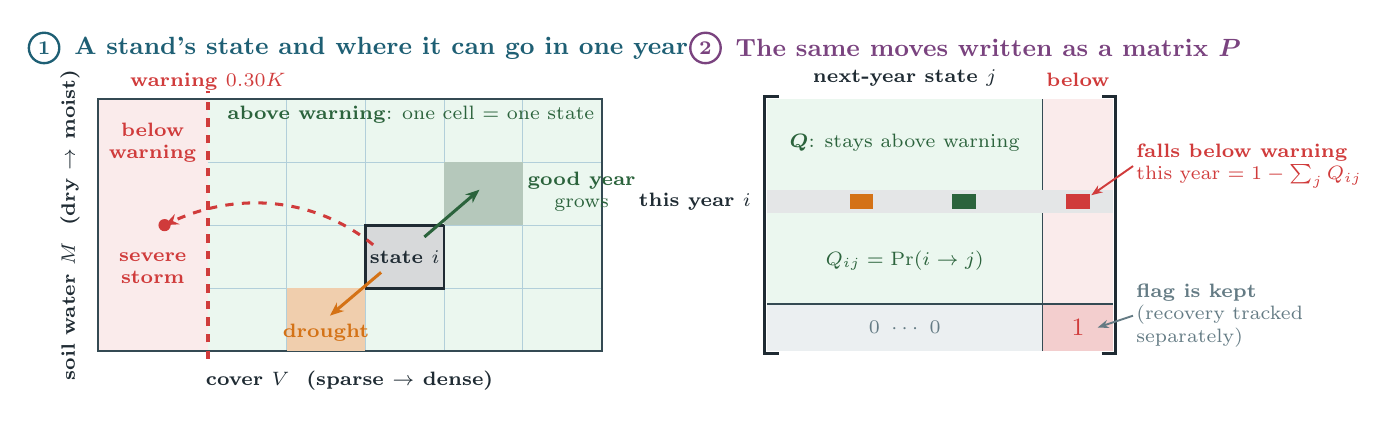
\begin{tikzpicture}[font=\small]

% ============================== LEFT: states and moves ==============================
\node[badge=pWater] at (0.22,4.45) {1};
\node[font=\small\bfseries, text=pWater, anchor=west] at (0.48,4.45) {A stand's state and where it can go in one year};

% regions: x 0.9..7.3 (cover), y 0.6..3.8 (soil water); warning line at x=2.3
\fill[pLimit!10] (0.9,0.6) rectangle (2.3,3.8);
\fill[pVegLight!70] (2.3,0.6) rectangle (7.3,3.8);
\foreach \x in {3.30,4.30,5.30,6.30} \draw[pWaterMid!50, line width=0.4pt] (\x,0.6) -- (\x,3.8);
\foreach \y in {1.40,2.20,3.00} \draw[pWaterMid!50, line width=0.4pt] (2.3,\y) -- (7.3,\y);
\draw[pAxis, line width=0.7pt] (0.9,0.6) rectangle (7.3,3.8);
\draw[pLimit, dashed, line width=1.2pt] (2.3,0.5) -- (2.3,3.9);

\node[font=\scriptsize\bfseries, text=pInk] at (4.1,0.22) {cover $V$ \ (sparse $\rightarrow$ dense)};
\node[font=\scriptsize\bfseries, text=pInk, rotate=90] at (0.55,2.2) {soil water $M$ \ (dry $\rightarrow$ moist)};
\node[font=\scriptsize\bfseries, text=pLimit] at (2.3,4.02) {warning $0.30K$};
\node[lab=pLimit] at (1.6,3.25) {\textbf{below}\\\textbf{warning}};
\node[lab=pVeg, anchor=north east] at (7.25,3.75) {\textbf{above warning}: one cell = one state};

% current cell i
\fill[pInk!18] (4.30,1.40) rectangle (5.30,2.20);
\draw[pInk, line width=1pt] (4.30,1.40) rectangle (5.30,2.20);
\node[font=\scriptsize\bfseries, text=pInk] at (4.80,1.80) {state $i$};

% three typical moves
\fill[pVeg!35] (5.30,2.20) rectangle (6.30,3.00);
\draw[mv=pVeg] (5.05,2.05) -- (5.75,2.65);
\node[lab=pVeg, anchor=west] at (6.32,2.62) {\textbf{good year}\\grows};

\fill[pPV!35] (3.30,0.60) rectangle (4.30,1.40);
\draw[mv=pPV] (4.50,1.60) -- (3.85,1.05);
\node[lab=pPV, anchor=north] at (3.80,0.98) {\textbf{drought}};

\draw[mv=pLimit, dashed] (4.40,1.95) .. controls (3.6,2.6) and (2.6,2.6) .. (1.75,2.2);
\fill[pLimit] (1.75,2.2) circle (2.2pt);
\node[lab=pLimit] at (1.6,1.65) {\textbf{severe}\\\textbf{storm}};

% ============================== RIGHT: the matrix ==============================
\begin{scope}[xshift=8.4cm]
\node[badge=pPlum] at (0.22,4.45) {2};
\node[font=\small\bfseries, text=pPlum, anchor=west] at (0.48,4.45) {The same moves written as a matrix $\bm P$};

% matrix box x 1.0..5.4, y 0.6..3.8 ; split x=4.5, y=1.2
\fill[pVegLight!70] (1.0,1.2) rectangle (4.5,3.8);
\fill[pLimit!10]   (4.5,1.2) rectangle (5.4,3.8);
\fill[pGrid!80]    (1.0,0.6) rectangle (4.5,1.2);
\fill[pLimit!25]   (4.5,0.6) rectangle (5.4,1.2);
\draw[pAxis, line width=0.7pt] (4.5,0.6) -- (4.5,3.8);
\draw[pAxis, line width=0.7pt] (1.0,1.2) -- (5.4,1.2);
\draw[pInk, line width=1.1pt] (1.15,0.57) -- (0.97,0.57) -- (0.97,3.83) -- (1.15,3.83);
\draw[pInk, line width=1.1pt] (5.25,0.57) -- (5.43,0.57) -- (5.43,3.83) -- (5.25,3.83);

% row i with three coloured entries matching the left panel
\fill[pInk!12] (1.0,2.35) rectangle (5.4,2.65);
\fill[pPV]   (2.05,2.40) rectangle (2.35,2.60);
\fill[pVeg]  (3.35,2.40) rectangle (3.65,2.60);
\fill[pLimit](4.80,2.40) rectangle (5.10,2.60);
\node[font=\scriptsize\bfseries, text=pInk, anchor=east] at (0.92,2.50) {this year $i$};

\node[font=\scriptsize\bfseries, text=pInk, anchor=south] at (2.75,3.84) {next-year state $j$};
\node[font=\scriptsize\bfseries, text=pLimit, anchor=south] at (4.95,3.84) {below};

\node[lab=pVeg] at (2.75,3.25) {$\bm Q$: stays above warning};
\node[lab=pVeg] at (2.75,1.75) {$Q_{ij}=\Pr(i\to j)$};
\node[lab=pGreyDark] at (2.75,0.90) {$0\ \cdots\ 0$};
\node[font=\small\bfseries, text=pLimit] at (4.95,0.90) {$1$};

% callouts
\node[lab=pLimit, anchor=west, align=left] (c1) at (5.65,2.95) {\textbf{falls below warning}\\this year $=1-\sum_j Q_{ij}$};
\draw[-{Stealth[length=4pt]}, pLimit, line width=0.7pt] (c1.west) -- (5.12,2.58);
\node[lab=pGreyDark, anchor=west, align=left] (c2) at (5.65,1.05) {\textbf{flag is kept}\\(recovery tracked\\separately)};
\draw[-{Stealth[length=4pt]}, pGreyDark, line width=0.7pt] (c2.west) -- (5.20,0.90);
\end{scope}

\end{tikzpicture}
\end{document}
